\documentclass[]{article}
\usepackage[T1]{fontenc}
\usepackage[utf8]{inputenc}
\usepackage[french]{babel}
\usepackage[]{graphicx}
\usepackage[]{hyperref}

\title{Bilan de projet}
\author{
    Théo Delmas\\
    Lauric Teysseyre\\
    Pierre-Louis Renon\\
    Julien Wattier\\
    \\
    Université Paul Sabatier\\
    Master Informatique 1\\
   } 

\begin{document}
\maketitle
\newpage
\tableofcontents
\newpage

\begin{section}{Objectif du document}
 Ce document présente le bilan du projet.
\end{section}

{
\setlength{\parindent}{0pt} %Retire les alinéas
\begin{section}{Référentiel initial}
 \begin{subsection}{Produits initiaux}
     Le product breakdown initial ainsi que les méthodes de réalisation étaient les suivants :

     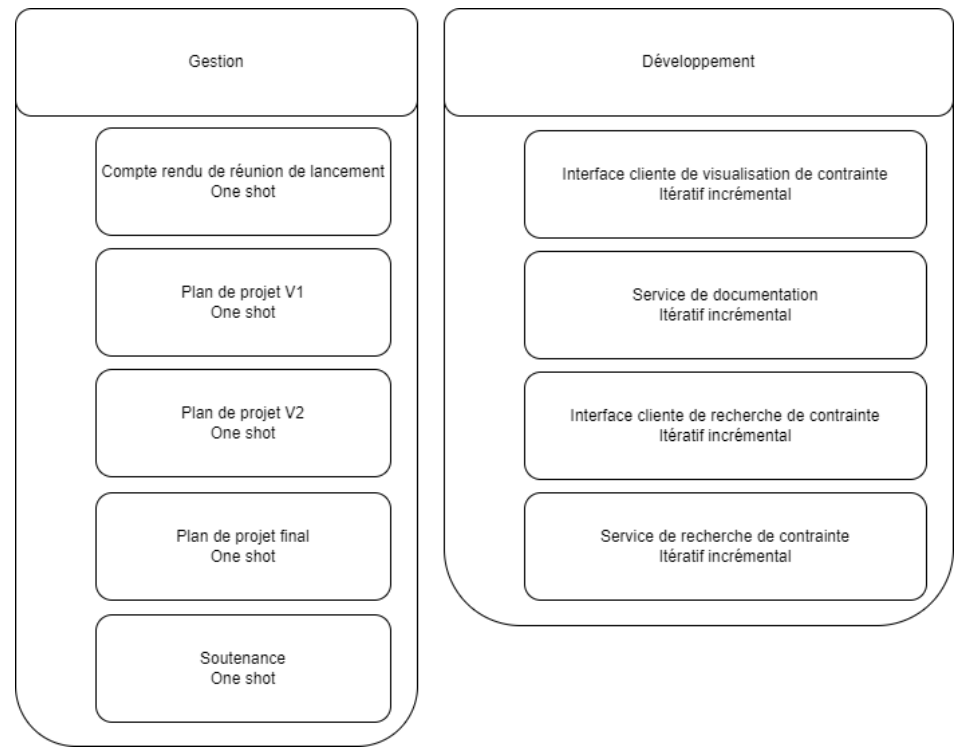
\includegraphics[scale=0.6]{IMG/PBS_initial}
 \end{subsection}
\end{section}

\begin{section}{État courant à la terminaison}
 \begin{subsection}{Produits réalisés}
     L’état des produit à la terminaison du projet sont exposés dans le schéma ci-dessous. Le code couleur indique leur état selon le code suivant :

     \begin{itemize}
         \item Vert : Le produit a été réalisé.
         \item Jaune : Le produit va être réalisé.
         \item Rouge : Le produit n’a pas été réalisé.
     \end{itemize}

     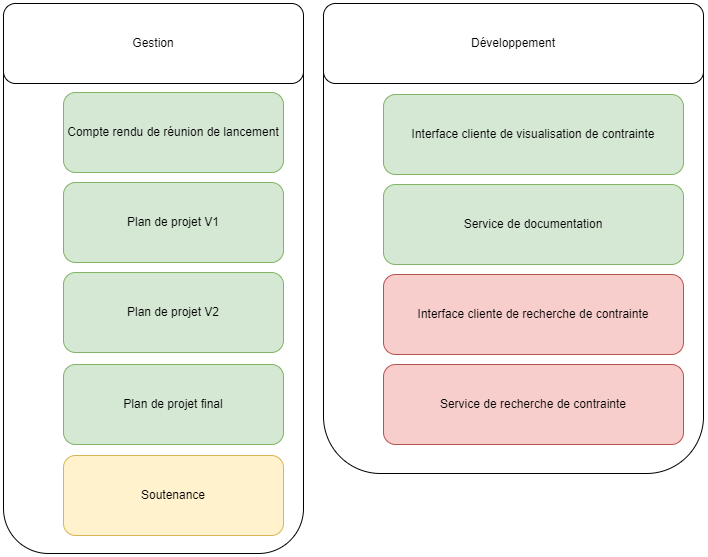
\includegraphics[scale=0.49]{IMG/PBS_final}

     La soutenance va être produit après la clôture du plan projet fixé au 14/03/2023.

     Concernant les produits liés au système de recherche de contrainte, il a été décidé début mars et avec accord du client qu’ils ne seraient pas produits faute de temps.
 \end{subsection}

 \begin{subsection}{Listes des événements}
     Le \href{Registre_des_faits_marquants.pdf}{registre des faits marquants} référence l'ensemble des événements ayant affecté le projet.
 \end{subsection}

 \begin{subsection}{Listes des décisions}
     Conformément à la gestion des décision du plan de projet, le \href{Registre_des_décisions.pdf}{registre des décisions} référence l'ensemble des décisions ayant amendé le plan de projet.
 \end{subsection}

 \begin{subsection}{Listes des livrables de gestion}
     L'ensemble des livrables de gestion sont disponibles sur ce \href{https://github.com/Szyckaa/UE-PROJET-DOCS-GESTION}{dépot github}, en consultant les releases.
 \end{subsection}

 \newpage

 \begin{subsection}{Listes des livrables de développement}
     L'ensemble des livrables de développement sont disponibles sur le \href{https://framagit.org/flopedt/FlOpEDT}{dépot framagit du projet}. Conformément à notre gestion des livrables, les livrables sont intégrés dans la \href{https://framagit.org/flopedt/FlOpEDT/-/tree/catalog}{branche catalog}.
 \end{subsection}
\end{section}

\begin{section}{Analyse du déroulement du projet}

 \begin{subsection}{Analyse de performance}
     L'\href{Analyse_de_performance.ods}{analyse de performance} récapitule les tâches, leur date d'enregistrement et leur date de réalisation. L'analyse présente également le nombre de tâches réalisées par sprint.

     Cependant ces indicateurs construit à posteriori ne sont pas pertinents car sur les premiers sprints l'équipe n'était pas rigoureuse concernant la gestion du projet et la plupart des tâches de cette période ont été ajoutés bien après leur identification et leur réalisation.

     D'autre part les tâches ne sont pas homogène dans la complexité de leur réalisation, certaines étant très courtes et d'autre bien plus longues.
 \end{subsection}

 \begin{subsection}{Maitrise partielle des technologies imposées }
     L'équipe avait une bonne expérience avec le framework front-end VueJS, imposé dans ce projet.

     Cela a permit un développement plus rapide, notamment pour que la nouvelle application s'intègre sur l'existant qui n'utilise pas VueJS.
 \end{subsection}

 \begin{subsection}{Des communications efficaces}
     L'ensemble des communications a globalement bien été géré.

     D'une part les communications internes qui consistaient à avoir l'ensemble des fournisseurs en vocal sur discord a permit un développement efficace puisqu'en cas de problème, un développeur était immédiatement aidé. Cela a également fortement augmenté la cohésion de l'équipe qui malgré la distance était toujours en contact.

     Concernant les communications avec le clients, elles se faisaient essentiellement lors des revues de sprint qui étaient tenues toutes les deux semaines, ce qui s'est révélé être un bon rythme au vu du projet, permettant de s'assurer de la conformité entre les besoins du client et la réalisation.

     D'autre part le client était très disponible pour des discussions plus informelles qui permettaient d'affiner rapidemment des besoins s'étant révélés trop flous.
 \end{subsection}

 \begin{subsection}{Un manque de contrôle}
     L'équipe n'a appliqué presque aucune contrôle des activités ou des produits.
     \begin{subsubsection}{Faute d'indicateur}
         Aucune indicateur n'existe permettant d'évaluer les activités et produits du projet. De fait elle ne peut faire de mesure sur le temps des ces indicateurs et les analyser.
     \end{subsubsection}

     \begin{subsubsection}{Faute de processus dédié}
         D'autre part, aucun processus clairement défini n'a été mis en place afin de contrôler les différentes activités du projet.
     \end{subsubsection}

     La principale conséquence est que faute de moyen de visualiser quantitativement la qualité des différentes activités et produits, la qualité de manière générale n'a que peu de sens dans ce projet. D'autre part l'absence d'activité de contrôle peut permettre une déviation du projet sans que l'équipe ne se rende compte.
 \end{subsection}

 \begin{subsection}{Baisse de production sur la fin du projet}
     L'équipe a connu une baisse du production sur la fin du projet. Les raisons sont que d'une part la motivation générale s'est érodée. D'autre part la réalisation des premiers produits et l'abandon des suivants faute de temps à relaxer l'équipe qui s'est alors permise de ralentir son rythme à tord.
 \end{subsection}

 \begin{subsection}{Manque de connaissance du fonctionnement de l'application}
     Au milieu du projet l'équipe a appris que le projet dans sa globalité utilisait une convention peu courante consistant à partir du principe que si une liste d'objet du système est vide c'est qu'en réalité elle désigne toute les instances de la classe de ces objets.

     Si l'adaptation ne nous a pas posé de problème, cela révèle que nous n'avions pas une connaissance suffisante des systèmes impactés par nos développement.
 \end{subsection}

 \begin{subsection}{Peu de conception}
     L'équipe n'a pas suffisament insisté sur les phases de conception et avait tendance à directement expérimenter des solutions en codant plutôt qu'en analysant le problème et en modélisant des solutions.

     De fait l'équipe à certainement manqué de recule et donc réduit la qualité des artéfacts produits.
 \end{subsection}

 \begin{subsection}{L'installation de l'environnement de travail compliquée}
     L'équipe a eu de nombreuses difficultés pour installer le serveur de développement car elle pensait pouvoir utiliser Docker mais il s'est révélé que le projet ne maintenanait plus le nécessaire pour fonctionner sous Docker.

     Par la suite, elle a eu quelques problèmes car une partie des développeurs utilisaient WSL plutôt qu'une vrai machine virtuelle pour le serveur.

     Tout celà a rendu le sprint 0 plus long et donc fait perdre du temps au projet.
 \end{subsection}

 \begin{subsection}{Un contexte difficile}
     Pour rappel le projet dans sa globalité est en train de découpler son back, réalisé avec Django, de son front qui jusque là était géré également par Django pour migrer vers VueJS. Dans ce contexte le client nous a demandé de réaliser les nouvelles fonctionnalités en utilisant les nouvelles technologies.

     Malheureusement celà a été compliqué car les fonctionnalités développés reposent sur du code existant qui n'utilise pas VueJS. Il a donc fallu mettre en place divers mécanismes pour s'intégrer sur l'existant, ce qui a compliqué le développement des fonctionnalités.
 \end{subsection}

 \begin{subsection}{L'évolution de la gestion}
    Il faut savoir que nous avons commencer le projet sans avoir de plan de projet, ni de connaissances sur la gestion de projet. De fait nous avons du élaborer les règles et processus au fur et à mesure, et donc changer nos méthodes de travail. 
    
    Cela nous a grandement impacté car nous avons régulièrement pris conscience que certains processus auraient dû être appliqué dès le début du projet, créant une certaines frustration impactant le moral.
 \end{subsection}

 \begin{subsection}{Une montée en compétence}
     L'équipe a connu un bonne montée en compétence, aussi bien sur le plan technique avec Django, VueJS, git et yarn, que sur le plan de la gestion et l'agilité en ayant appliqué une partie des processus agiles usuels.

     D'autre part elle a découvert l'outil Liveshare permettant de faire du peer-programming et qui s'est révélé très utile pour débboger ou réaliser les revues de code.
 \end{subsection}

 \newpage

 \begin{subsection}{Aucune définition du protocol de traitement des besoins et du test}
     L'équipe n'a jamais défini un protocole de traitement des besoins précisant qu'elle devait s'assurer qu'un besoin passe en "Ok" (Done) avant d'en traiter un autre étant en "A faire". De fait elle s'est permise d'enchaîner la réalisation des besoins sans les tester, se disant qu'elle pourrait le faire vers la fin du projet. Elle a donc accumuler une forte dette technique qu'elle n'a pu rattraper dans les temps.

     D'autre part elle n'a pas définie le protocol de test dès le début, encore une fois persuadée qu'elle pourrait le faire sur la fin du projet, ce qui l'a inciter à enchaîner la réalisation sans tester, et donc à accumuler de la dette technique.
 \end{subsection}

 \begin{subsection}{Un gestion du besoin initialement trop faible}
     Au début du projet l'équipe ne produisait pas de rapport de réunion qui mettent en relief les actions à effectuer pour le projet. De fait les tâches à effectuer n'étaient pas forcément mise à jour dans l'immédiat et certaines ont été temporairement oubliées.

     Cela n'a que peu impacté le projet car les tâches oubliées n'étaient pas prioritaires mais cela aurait pu grandement impacter les artefacts produits en créant une différence entre ce qu'attendait le client et ce que produisait l'équipe.
 \end{subsection}
\end{section}

\begin{section}{Leçons apprises}
 \begin{subsection}{L'importance de la phase d'initialisation du projet}
    La phase d'initialisation est l'occasion de définir rigoureusement les différents processus et règles appliqués par l'équipe. Cette base évoluant par la suite selon les besoins. Dans de véritable projet avoir un définition initiale rigoureuse nous semble essentielle pour la bonne conduite du projet.

    Dans le cas de projet d'extension, c'est durant cette phase que l'équipe chargée de la réalisation devrait s'imprégner du projet à modifier en comprenant comment fonctionnent les différents systèmes qui vont être impactés.
 \end{subsection}

 \begin{subsection}{L'importance du contrôle}
    Le controle permet d'assurer la qualité du projet en analysant des indicateurs pertinents qui sont produits tout au long du projet.
    
    Il nous parait évident que ces processus auraient ajouté une plus value au projet en nous permettant de l'évaluer quantitativement que qualitativement, et donc prendre des décisions pertinente au regard des résultats des analyses. Cette classe de processus n'est donc pas a négliger.
 \end{subsection}

 \begin{subsection}{L'importance des communications}
    La forte communication avec le client semble être un point plus que bénéfique dans le cadre des projets agiles afin de valider l'adéquation entre un besoin et sa réalisaton. D'autre part elle évite la déviation du projet.

    Concernant les communications internes, elle ont eu un double intérêt dans ce projet puisqu'elle ont renforcé la cohésion de l'équipe tout en évitant les situations de blocages des développeurs.
 \end{subsection}
\end{section}

\begin{section}{Perspectives}
 \begin{subsection}{Insister sur la conception}
     En maintenant des schémas UML des productions et de l'existant impacté, l'équipe pourrait bénéficier d'une vision globale du problème au moment de réaliser les tâches. De là, elle pourait ainsi modéliser diverses solutions et sélectionner celle respectant au mieux nos exigences. Le développements des fonctionnalités serait certainement plus efficace ainsi.
 \end{subsection}

 \begin{subsection}{Définition rigoureuse du traitement des besoins}
    En définissant dès le départ un protocole de traitement des besoins qui minimise l'accumulation de dette technique, l'équipe pourrait produire des artéfacts de meilleure qualité. Dans le cadre de se projet, ce protocole aurait du spécifier qu'il était interdit de traiter un nouveau besoin dans que celui actuellement traité ne devenait pas "Done", et donc au passage bien définir "Done". Ainsi il n'y aurait pas eu d'absence de test et donc une telle dette technique.
 \end{subsection}

 \begin{subsection}{Appliquer du contrôle}
    L'équipe devrait produire dès le début des indicateurs qui serait maintenu à jour durant tout le projet. L'intérêt serait double : d'une part, se rendre compte si un des aspect du projet dévie. D'autre part, permettre l'optimisation du fonctionnement de l'équipe en prenant des décisions rationnelles basées sur ces indicateurs.  
 \end{subsection}
\end{section}

\begin{section}{Recommandations}
 \begin{subsection}{Migrer avant d'étendre}
     Pour rappel l'application est actuellement en train de migrer d'une application monolothique Django vers un front VueJS et un back Django dissociés. Notre travail consistait à étendre l'application en ajoutant un système. Au vu du contexte le client souhaitait que les nouveaux développements respectent la nouvelle philosophie de front et back dissociés.

     Malheureusement cela a rendu nos développements compliqué en nous forçant à nous adapter à un code qui est voué à disparaître, notamment côté front. Nous pensons donc que la migration devrait être effectuée ; ou du moins bien entammée ; avant de réaliser de nouvelles extensions.
 \end{subsection}

 \begin{subsection}{Documentation du code source}
     L'équipe qui maintient le projet devrait mettre en place une documentation assez généraliste qui décrit qu'est ce que chaque partie du projet réalise en ajoutant des markdowns dans les différents dossiers du projet. Cette absence de documentation est un frein pour les nouveaux arrivants, et semble essentiel sachant que le projet est open-source.
 \end{subsection}
\end{section}

}
\end{document}